\chapter{Propuesta de Solución}
El análisis de la opción \emph{reuseport} efectuado en el capítulo anterior reveló que es posible obtener mejores tiempos en el consumo de datos desde una interfaz de red con respecto al consumo tradicional. Ahora bien, los aspectos negativos reconocidos en el uso de ésta opción nos motivan a diseñar e implementar una propuesta de solución que satisfaga ciertos requerimientos puntuales, en pos de ubicarla como una opción viable --y preferible por sobre reuseport-- en un uso en entornos como el propuesto.

En el presente capítulo se formalizan los requerimientos mínimos que constituyen nuestra solución ideal, los cuales servirán como lineamientos mínimos a satisfacer por nuestra solución. Con dicho marco de requisitos, se construye un modelo para esquematizar el funcionamiento de la solución propuesta. Posteriormente se trabaja en la especificación de la implementación de la solución, para terminar con una evaluación final de performance bajo los mismos entornos que las pruebas desarrolladas a lo largo de la investigación y concluir determinando si existen beneficios reales asociados a nuestra propuesta con respecto a otras alternativas.

\section{Formalización de Requerimientos}
Como se ilustró en el capítulo anterior, la alternativa de \emph{reuseport}, desarrollada para mejorar la performance de las estructuras sockets en el kernel de Linux se caracteriza por ser complejas en su funcionamiento ya sea por su implementación para funcionar sobre aplicaciones ya desplegadas en un sistema, o por quebrantar ciertos principios de programación definidos --como los sugeridos por el modelo estándar OSI-- con consecuencias como tener que modificar el código de programas ya operativos bajo el modelo tradicional. Existen otras alternativas para emular un comportamiento similar a la técnica de reuseport como lo es la utilidad de \textbf{IPTables} \cite{book:iptables} la cual se caracteriza por su dificultad de uso y configuración, haciéndola difícil de sugerir en entornos delicados de producción. El objetivo de la presente sección es caracterizar las especificaciones ideales que debe satisfacer un desarrollo enfocado en brindar una optimización de la operación de los sockets de Linux, en el marco de la preservación de características deseadas especificadas por el ya mencionado modelo OSI.

En función de lo anterior, a continuación se especifican las propiedades estructurales que debe contemplar una solución ideal:

\begin{description}
\item[Rendimiento] El requerimiento principal para la solución objetivo constituye el garantizar un buen rendimiento. La solución debe poder brindar mejores tiempos de operación que el enfoque tradicional de consumo de datos desde un socket, y han de ser tiempos --a lo menos-- competitivos con la mejor alternativa evaluada a lo largo de la investigación en curso, que corresponde al rendimiento obtenido con el mecanismo de \emph{Reuseport}.
\item[Bajo Overhead] A fin de lograr una solución con bajo  nivel de sobrecarga e impacto con el resto del sistema se debe procurar considerar una alternativa que opere en los niveles más bajos del sistema operativo, a fin de evitar la sobrecarga efectuada por concepto de interrupciones o intervenciones que son propias de soluciones que operan en espacio de usuario.
\item[Modularidad] El esquema ideal debe ser modular, en el sentido de garantizar una sencilla instalación y remoción de la misma en un sistema sin necesitar significativas dependencias para con otros componentes a modo de garantizar amplia compatibilidad entre sistemas. En otra arista de este mismo requerimiento, se busca desarrollar una solución que permita modificaciones en sí misma de manera sencilla a fin de garantizar \textbf{extensibilidad}.
\item[Adaptabilidad] Finalmente, una propiedad que debe contemplar la solución es ser fácilmente configurable y adaptable a los distintos entornos y requerimientos que se presenten en línea con las necesidades de rendimiento que se persigan.
\end{description}

Las características antes mencionadas se utilizaron como requerimientos estructurales en lo que se postula como nuestra propuesta de diseño de solución.

\section{Modelo de Funcionamiento de la Solución}
Tomando en consideración los requerimientos descritos en la sección anterior, se optó por una solución cuyo modelo de funcionamiento fuese como el descrito en la imagen \ref{fig:modeloUDPRedistribuyeModule}, construido como un \textbf{módulo del kernel} capaz de intervenir paquetes de Internet de las características que atañen éste estudio, y los redistribuyan entre un pool de nuevos puertos para luego ser atendidos por interfaces sockets exclusivas en cada caso. Para una primera versión de ésta solución se postularon 2 esquemas de distribución que se describen en apartados posteriores.

	\begin{figure}[!h]
		\centering
		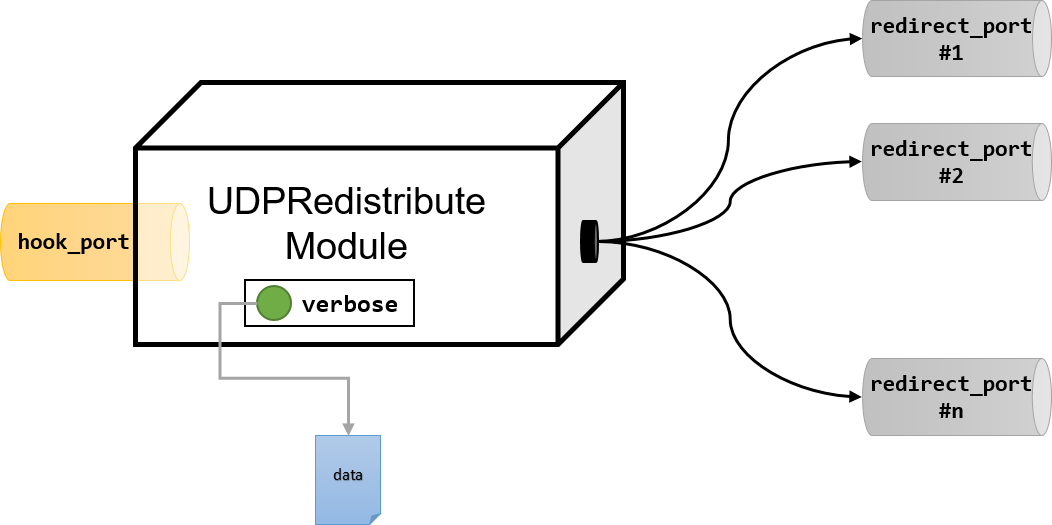
\includegraphics[scale=.55]{imagenes/udpredistributemoduleDiagram.png}
		\caption{Diagrama esquemático de la operación de la solución propuesta.}
		\label{fig:modeloUDPRedistribuyeModule}
	\end{figure}

Ésta decisión de diseño se fundamenta en que con éste enfoque se satisfacen prácticamente todos los requerimientos definidos en la sección anterior: En primer lugar es un enfoque que añade \textbf{bajo overhead} al sistema. Al ser un módulo, la solución se ejecuta en el espacio del kernel por lo que cuenta con privilegios que evitan la sobrecarga experimentada por soluciones en espacio usuario, además de tener un bajo impacto para otras aplicaciones por no intervenirlas en su operación. Segundo, siendo un módulo, al momento de instalarlo en el sistema se pueden especificar distintas configuraciones pertinentes al modo de funcionamiento deseado, permitiendo un amplio grado de \textbf{adaptabilidad} de acuerdo al entorno y resultado deseado. En tercer lugar, al ser un módulo es fácilmente \textbf{modificable} permitiendo añadir, modificar o eliminar del mismo toda la lógica de programación implementada en su interior. Para ello sólo basta modificarlo, recompilarlo e instalarlo nuevamente. De la mano con lo anterior, es fácilmente removible del sistema.

Las componentes que rigen el modelo en su operación ilustrados en la imagen \ref{fig:modeloUDPRedistribuyeModule} se describen acuerdo a las siguientes definiciones:


\begin{description}
\item[hook\_port] Valor que determina el puerto a interceptar para la redirección de paquetes.
\item[redirect\_port] Colección de valores que indican los puertos hacia los cuales redistribuir los paquetes interceptados y modificados.
\item[verbose] Índice del grado de detalle con que se guardarán registros de acción del módulo en los mensajes del kernel.
\end{description}

En la práctica, la operación de la solución propuesta se inspira en el mecanismo de un \emph{proxy}, modificando solamente los valores en las cabeceras de los paquetes intervenidos. El modelo implementa la siguiente lógica de instrucciones:

\begin{enumerate}
\item Interceptar paquetes de tipo UDP y que estén dirigidos a un determinado puerto (\textbf{hook\_port}).
\item Modificar el paquete, actualizando valores como el \emph{checksum} del mismo.
\item Redireccionar el paquete, modificando el puerto de destino del paquete (\textbf{redirect\_port}) de acuerdo al esquema de distribución operativo.
\item Reincorporación del paquete modificado en el tránsito de distribución del kernel por la vía ordinaria.
\end{enumerate}

Por su naturaleza de acción, la solución opera estrictamente entre las capas de Red y de Transporte en el modelo OSI, interviniendo esos niveles de abstracción a través de la modificación de los encabezados correspondientes al empaquetamiento por los protocolos IP y UDP respectivamente.


\subsection{Esquemas de Distribución}
Como ya se mencionó, la solución desarrollada comprende una etapa de reparto de paquetes de acuerdo a distintos esquemas de distribución. En este contexto, un esquema de distribución se define como un conjunto de reglas para reasignar los paquetes interceptados entre un pool de puertos previamente definidos. En la versión desarrollada de la solución se implementaron 2 esquemas de distribución: \emph{RandomSched} y \emph{SequentialSched}.

\subsubsection{RandomSched}
El esquema de distribución \emph{RandomSched} realiza una distribución entre puertos de manera aleatoria. La aleatoriedad de éste esquema se consigue por medio de la llamada de sistema \verb=get_random_bytes()= que sugiere una entrega aleatoria de resultados en valores de bytes. Dicho resultado se emplea para la redistribución de los paquetes de acuerdo a la aplicación de una operación de módulo sobre el valor aleatorio obtenido, por la cantidad total de puertos objetivos de redistribución. El valor resultante indica el índice del puerto (entre los puertos de redirección) a utilizar. La utilización de dicha función se justifica en ser uno de los mecanismos más sencillos de obtener aleatoriedad en demanda en el espacio del kernel y que, según su documentación, sus valores generados siguen una distribución uniforme.


\begin{figure}[th!]
\centering
\subfigure[]{
	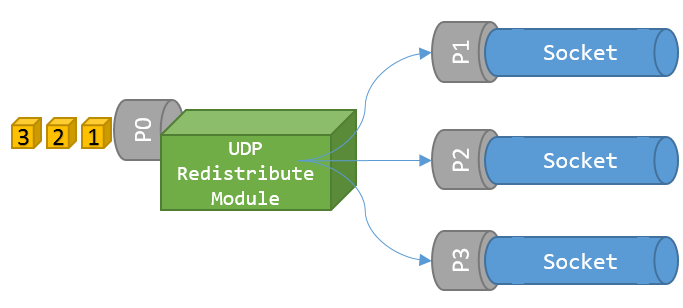
\includegraphics[width=.3\textwidth]{imagenes/rand1.png}
}
\subfigure[]{
	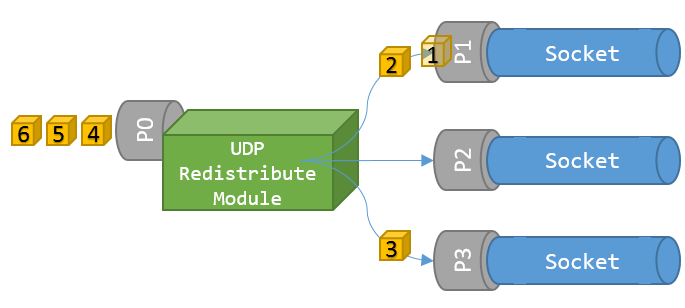
\includegraphics[width=.3\textwidth]{imagenes/rand2.png}
}
\subfigure[]{
	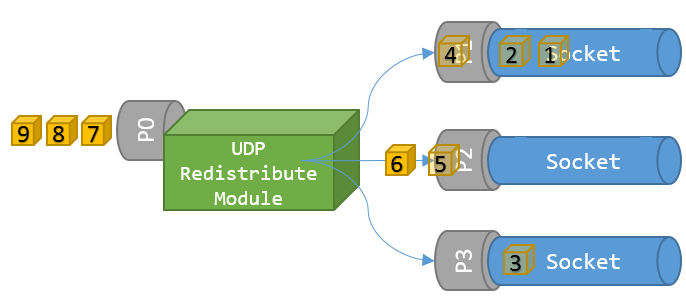
\includegraphics[width=.3\textwidth]{imagenes/rand3.png}
}
\caption{Evolución en la distribución de paquetes usando el esquema aleatorio por \emph{RandomSched}.}
\label{fig:RandomSched}
\end{figure}

A pesar de que en teoría éste esquema en promedio promete una distribución uniforme, en la práctica es posible que la carga no sea en efecto perfectamente distribuida por lo que éste esquema es práctico en escenarios donde se permita cierta entropía en la reasignación de carga entre puertos de destino.

\subsubsection{SequentialSched}
El segundo esquema de distribución diseñado es denominado \emph{SequentialSched}. En éste caso, se hace una distribución secuencial entre los distintos puertos de destino de distribución asignados en el módulo. De ésta manera, éste esquema consigue una perfecta distribución entre puertos de redirección logrando una carga equitativa entre todos ellos.

\begin{figure}[th!]
\centering
\subfigure[]{
	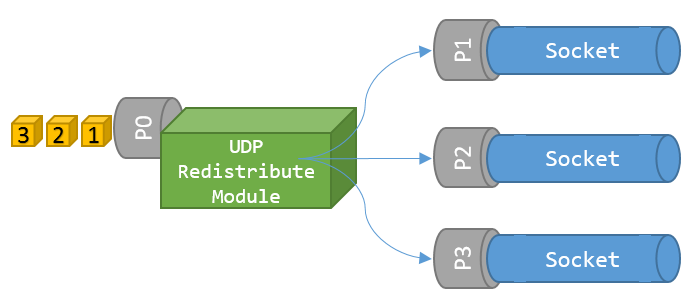
\includegraphics[width=.3\textwidth]{imagenes/seq1.png}
}
\subfigure[]{
	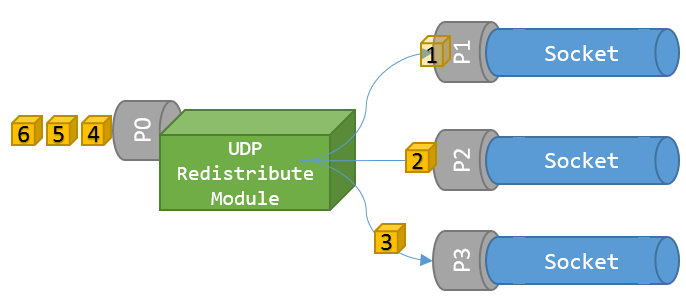
\includegraphics[width=.3\textwidth]{imagenes/seq2.png}
}
\subfigure[]{
	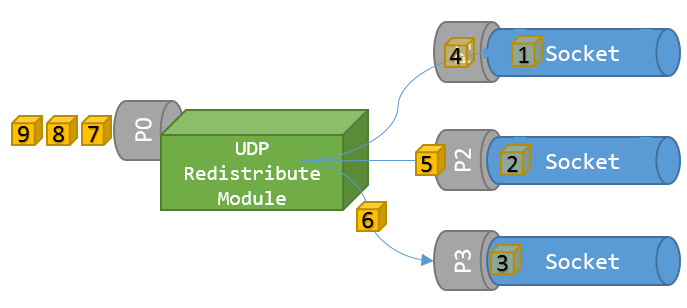
\includegraphics[width=.3\textwidth]{imagenes/seq3.png}
}
\caption{Evolución en la distribución de paquetes usando el esquema secuencial por \emph{SequentialSched}.}
\label{fig:SequentialSched}
\end{figure}

\section{Implementación}
El mecanismo de funcionamiento planteado en la sección anterior postula modificar el destino final de los paquetes, a través de la modificación de los encabezados de los paquetes interceptados cambiando el valor del puerto de destino de los mismos. Dicha operación implica dos características a considerar:

\begin{enumerate}
\item Interceptar paquetes en el momento apropiado. A priori dicho momento sería idealmente apenas el sistema reconozca el arribo de un paquete y sin intervención de otros mecanismos del sistema.
\item Modificar paquetes para su redirección. La información de puerto de destino es una especificación propia de la capa de transporte según el modelo OSI por lo que dicha información es inherente a los encabezados de dicha capa.
\end{enumerate}

Dados los requerimientos anteriores, para la implementación de la solución se optó por el diseño de un módulo del kernel operacional sobre el framework de \emph{Netfilters} del kernel, el cual permite intervenir paquetes de las características relacionadas al caso de estudio y brinda la flexibilidad para modificar los encabezados de los mismos, logrando el efecto de redistribución entre distintos puertos, y siendo lo suficientemente flexible como para emplear distintos esquemas de distribución para la redirección de los mismos. Además, al ser un módulo del kernel, existen diversas guías técnicas que profundizan los aspectos de diseño a considerar en construcción del mismo y al ser parte del módulo de red del kernel mismo, apoya el requerimiento de \textbf{adaptabilidad} solicitado en la sección de requisitos de la solución.

\subsection{NetFilter Framework}
Netfilter \cite{report:netfilterModule} es un framework disponible en el núcleo de sistemas Linux que permite la manipulación de paquetes en distintos niveles del tránsito de los mismos a través del stack de protocolos de red del kernel. Parte del módulo de red del mismo kernel de Linux, Netfilters provee una interfaz para implementar los denominados \emph{hooks}, funciones de intervención de paquetes donde se da la libertad de programar libremente operaciones sobre cada estructura de paquete intervenido. Los \emph{hooks} implementados deben ser registrados en el sistema en un \emph{punto de intercepción} y es el mismo kernel el encargado de incluirlos en su rutina de inspección de cada paquetes a medida que los mismos van llegando al sistema, aplicándolos de acuerdo a reglas de prioridad y puntos de intervención bien definidos. Netfilters es una de las herramientas más potentes para la manipulación de paquetes, siendo la base de distintas herramientas que operan en espacio usuario como por ejemplo IPTables.

Las capacidades de manipulación que provee Netfilters son sumamente potentes abarcando un amplio espacio de acción en el sistema, postulándose así como una interesante herramienta que contemplar en el desarrollo de la solución al desafío planteado.

\subsubsection{Arquitectura de Interrupción en Netfilters}
El framework provee una arquitectura de seguimiento de los distintos paquetes para interceptar que se modela en un esquema definido en la imagen \ref{fig:netfilterArchitecture}. Esta arquitectura es lo suficientemente amplia como para intervenir paquetes en distintos niveles de comunicación y tránsito a través del kernel.

\begin{figure}[!h]
	\centering
	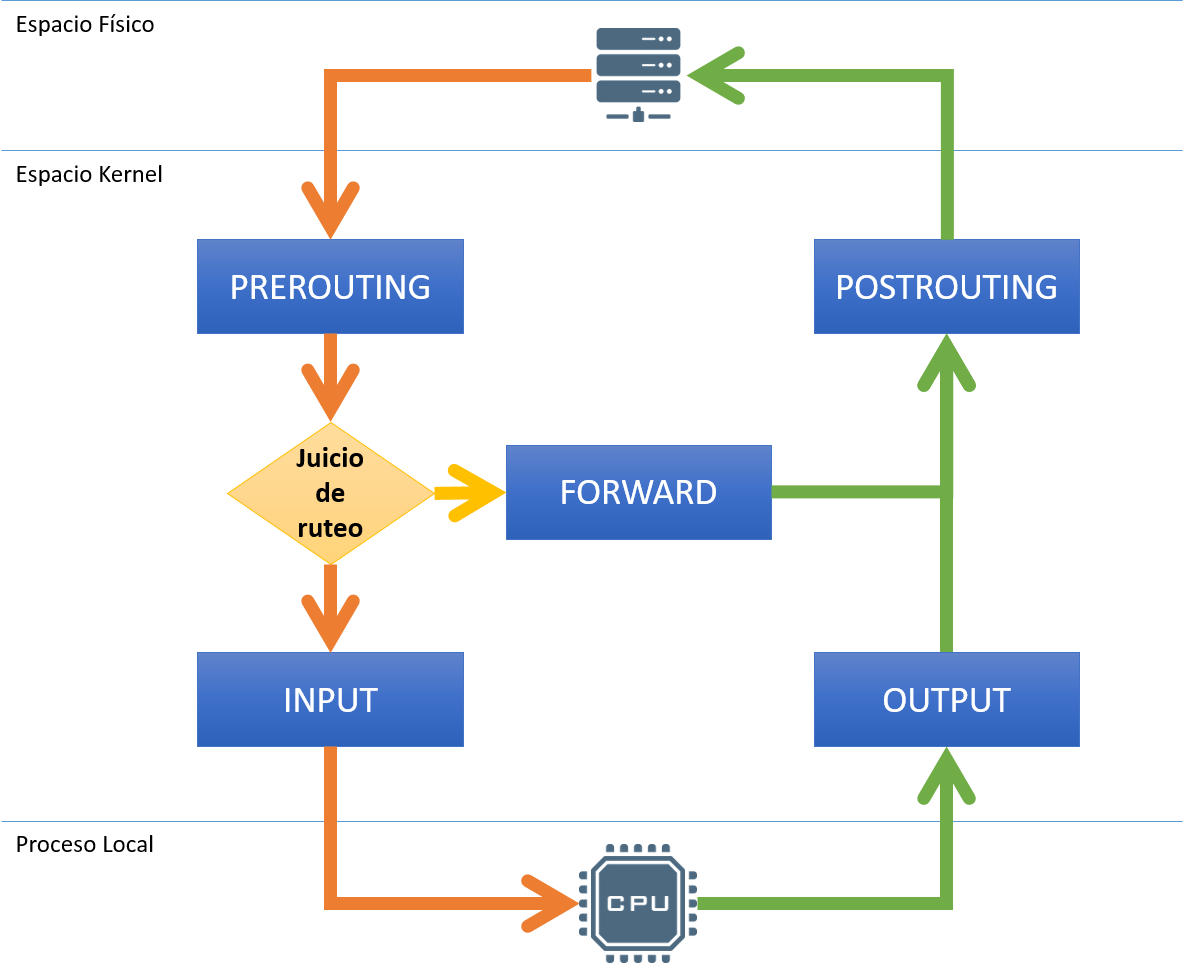
\includegraphics[scale=.65]{imagenes/netfilterArchitecture}
	\caption{Esquema de la arquitectura de interrupción disponible para la intervención de paquetes provisto por el Netfilters Framework.}
	\label{fig:netfilterArchitecture}
\end{figure}

El esquema ilustrado en la figura \ref{fig:netfilterArchitecture} da cuenta del flujo que recorre un paquete en el kernel en consideración de los modos de intervención que brinda el framework de Netfilters. Cada uno de los puntos ilustrados en dicho diagrama es un potencial punto de intervención, y da cuenta de alguna etapa en el arribo o salida de un paquete. Los distintos puntos de intervención disponibles en \emph{IPv4} que soporta Netfilters se detallan a continuación:

\begin{description}
\item[NF\_IP\_PRE\_ROUTING] Todos los paquetes entrantes pasan a través de éste hook, al momento de ejecutarse la llamada a sistema \verb=ip_rcv()=, antes de cualquier proceso de ruteo.
\item[NF\_IP\_INPUT] Todo paquetes destinado al equipo local pasa por éste hook, al ejecutarse la llamada \verb=ip_local_deliver()=.
\item[NF\_IP\_FORWARD] Todo paquete entrante que esté en tránsito a su destino final (es decir, que su destino final no sea el equipo local y sólo deba ser redirigido) pasa por éste hook, en la llamada a sistema \verb=ip_forward()=.
\item[NF\_IP\_OUTPUT] Todo paquete saliente creado en el equipo local, pasa por éste hook, en la llamada a sistema \verb=ip_build_and_send_pkt()=.
\item[NF\_IP\_POST\_ROUTING] Todo paquete saliente, haya sido creado en éste equipo o solo redirigido por él, pasa por éste hook, en la llamada a sistema \verb=ip_finish_output()=.
\end{description}

\subsubsection{Implementación de funciones de Interrupción usando Netfilters}
El framework en cuestión está diseñado para poder aprovechar sus funcionalidades fácilmente a partir de un módulo adicionado al kernel. Para ello, basta incluir las directivas de encabezados del framework en el módulo implementado (\verb=#include <linux/netfilter.h>=) e implementar los mecanismos de registro del \emph{hook} en el sistema, especificando sus opciones como: \textbf{prioridad}, \textbf{familia} y \textbf{punto de interrupción}. Para ésta tarea, se emplean valores constantes provistos por el mismo framework. Además de lo anterior, en el módulo se ha de implementar la función a aplicar sobre cada paquete intervenido, para lo cual es necesario seguir la convención que especifica el mismo framework, esto es, implementar un prototipo de función que propone el framework que se ilustra en el segmento de código \ref{code:netfilter}.

\vspace{1pc}
\begin{lstlisting}[style=CInputStyle, label=code:netfilter, captionpos=b, caption={Prototipo de la función de interrupción a ser definida en un \emph{hook} de Netfilters.}]
static unsigned int hook_func(
            		unsigned int hooknum,
            		struct sk_buff *skb, 
            		const struct net_device *in, 
            		const struct net_device *out, 
            		int (*okfn)(struct sk_buff *));
\end{lstlisting}

Dicho prototipo de función comprende 5 valores a recibir que contienen información relacionada al paquete que se ha de intervenir: \textbf{hooknum} Que corresponde al valor del mismo nombre que se asigna al momento de registrar la función de \emph{hook} y que hace referencia al punto de interrupción en que inspeccionará paquetes nuestro \emph{hook}. \textbf{skb} que es un puntero a una estructura tipo \verb=sk_buff= que almacena el paquete interceptado propiamente tal, y del cual se pueden extraer y modificar los encabezados de las capas de transporte y red para modificar el tránsito del paquete. Los punteros \textbf{in} y \textbf{out} de estructuras \verb=net_device= que apuntan a las interfaces de los dispositivos de red de procedencia y destino del paquete, registradas al momento de su interceptación, y \textbf{*okfn} (\emph{okay function}) que corresponde a una función que es invocada cuando todas las funciones registradas con éste hook retornan \verb=NF_ACCEPT=, significando que el paquete sigue en tránsito por el sistema.

Finalmente, las funciones de \emph{hook} deben especificar un valor de retorno que determina el camino a seguir por el paquete intervenido. En éste sentido, el framework especifica 5 posibles valores de retorno para las funciones de interrupción especificadas a continuación:
\begin{description}
\item[NF\_ACCEPT:] Para que el paquete prosiga su entrega, es decir, promueve el paquete a la siguiente etapa de distribución según módulo de red del kernel.
\item[NF\_DROP:] Para descartar el paquete, cancelando su entrega.
\item[NF\_STOLEN:] Para adueñarse del paquete. Es decir, sacar el paquete del entorno de Netfilters y brindarle su propiedad a la misma función de \emph{hook}.
\item[NF\_QUEUE:] Para encolar el paquete y poder manipularlo en espacio usuario.
\item[NF\_REPEAT:] Para llamar a la función de \emph{hook} en cuestión, otra vez.
\end{description}

\subsection{Implementación de la solución usando Netfilters}
Para el proceso de registro del \emph{hook} se tomaron ciertas consideraciones que permitieran garantizar la plena operatividad de la solución en el entorno de trabajo.

En primer lugar, se seleccionó como punto de interrupción del \emph{hook} a \verb=NF_INET_PRE_ROUTING=, ello pues corresponde al nivel más temprano de interrupción desde el arribo del paquete por la interfaz del sistema que admite el framework y básicamente captura todo tránsito de paquetes. Por la naturaleza de paquetes a trabajar se configuró la familia del \emph{hook} como \verb=PF_INET= que abarca a la familia de los protocolos de internet. Para el apartado de prioridad del \emph{hook} se seleccionó como el valor constante \verb=NF_IP_PRI_FIRST= provisto por el framework mismo y que garantiza la más pronta aplicación posible de nuestro \emph{hook} a los paquetes interceptados. Ésta decisión se apoya en que se desea el menor impacto para con otras componentes del sistema, por ello la intervención debe ser temprana y poco invasiva. Finalmente, se implementó el cuerpo de la función para tratar cada paquete interceptado (\verb=hook_func=) en la cual se realiza una inspección para reconocer los paquetes de interés en nuestro caso de estudio (paquetes de tipo UDP dirigidos al puerto configurado a interceptar) para luego modificar los encabezados y permitir al paquete su tránsito en el sistema.

\subsection{Código Fuente}
La solución\footnote{\url{https://github.com/sebablasko/UDPRedistributeModule}} fue elaborada siguiendo los principios de construcción de un módulo estándar de Linux \cite{report:netfilterModule}. Básicamente se implementaron los métodos \verb=init_module= y \verb=cleanup_module= para la instalación y eliminación del módulo respectivamente. Es en el primer método donde se gatilla la construcción y el registro del \emph{hook} definido para la interrupción de los paquetes. Para los procesos de registro y eliminación del \emph{hook} del sistema se usan respectivamente las llamadas \verb=nf_register_hook= y \verb=nf_unregister_hook= provistas por el framework de Netfilters.

\section{Instalación y Utilización}
Preservando la dinámica de un módulo de kernel, la solución requiere ser primero compilada y luego instalada en el sistema de acuerdo a los comandos tradicionales para dicho propósito de que dispone un sistema Linux.

\subsection{Compilación}
Para el proceso de compilación se requiere disponer tanto de los encabezados del kernel activo en la máquina a instalar, además de su código fuente. La gran mayoría de las distribuciones modernas de Linux incorporan mecanismos muy simples para poder obtener esos recursos sin mayores problemas.

La solución desarrollada incorpora un archivo \verb=Makefile= que resume las instrucciones para la compilación y correcta limpieza del mismo, utilizable en la mayoría de los escenarios sin necesidad de ningún cambio.

\subsection{Instalación y Configuración}
Una vez compilado, para la instalación en el sistema se deben emplear los comandos tradicionales de Linux para agregar módulos al kernel, específicamente \verb=insmod= para instalar. Es importante recordar que ésta es una operación que requiere privilegios en el sistema por lo que debe ser ejecutada en modo administrador.

Al momento de realizar la instalación se debe proveer la configuración que regirá la operación de la solución. La configuración consta de la incorporación de las siguientes opciones:

\begin{description}
\item[verbose] Para seleccionar un nivel de detalle en los mensajes que se dejarán en el registro del kernel sobre la actividad del módulo. Los niveles disponibles de verbosidad son:
\begin{description}
\item[verbose=0] Sólo registra la configuración de instalación y de operación del módulo.
\item[verbose=1] Registra lo mismo que el nivel de verbosidad 0, además de registrar para cada paquete correctamente interceptado detalles de la nueva dirección de puerto de destino que se ha asignado.
\item[verbose=2] Registra lo mismo que los niveles 0 y 1, además de informar para cada paquete capturado detalles de sus construcción como direcciones \verb=IP= y puertos de origen y destino, largo de encabezados y todos los pasos de modificación del paquete.
\end{description}
\item[hook\_port] Para configurar el puerto desde el cual se interceptarán los paquetes. Es decir, todo paquete que venga dirigido a éste puerto, pasará por el proceso de redistribución del módulo.
\item[start\_redirect\_port] Para configurar el puerto inicial que servirá para redirigir los paquetes interceptados.
\item[number\_redirect\_ports] Para determinar cuántos serán los puertos de redirección que se emplearán en el esquema de distribución del módulo.
\item[port\_sched] Para seleccionar el esquema de distribución a utilizar en la reasignación de puertos por paquete. Las opciones en éste caso son: 1 para \textbf{RandomSched} y 2 para \textbf{SequentialSched}.
\end{description}

En la práctica, los puertos de redirección quedan determinados a partir del valor de \verb=start_redirect_port= y hasta \verb=start_redirect_port + number_redirect_ports=.

\vspace{1pc}
\begin{lstlisting}[style=BashInputStyle,	breaklines=true, caption=Ejemplo de instalación de la solución, captionpos=b]
    # sudo insmod UDPRedistributeModule.ko verbose=2 hook_port=13131 start_redirect_port=1820 number_redirect_ports=4 port_sched={1,2}
\end{lstlisting}


\subsection{Utilización}
Una vez instalada, la solución queda plenamente operativa en el sistema llevando un registro de sus operaciones dependiendo del nivel de verbosidad definido al instante de la instalación. Es importante resaltar que es responsabilidad del usuario tomar posesión del conjunto de puertos de redirección definido en la solución, usándolos para los fines que él mismo desee.

\subsection{Eliminación}
La remoción de la solución desde el sistema es muy simple y se basa en que la misma es sólo un módulo del kernel, por lo tanto basta aplicar el comando \verb=rmmod= del sistema acompañado del nombre del módulo. Para una completa limpieza del módulo, es recomendable también limpiar los registros generados al momento de la compilación del módulo, para lo cual se puede ejecutar la directiva \verb=make clean= del archivo \verb=Makefile= provisto en la solución.

\section{Evaluación de Rendimiento de la Solución}

A fin de poder estudiar el funcionamiento y determinar el rendimiento de la solución propuesta, se construyó un experimento siguiendo la misma dinámica con que se valuaron los experimentos anteriores (Tanto el caso de estudio original como el nuevo caso de estudio de \emph{Reuseport}). De esta manera, se construyó un nuevo caso de estudio (Ver figura \ref{ fig:casoPruebaModulo}) basado en el mismo experimento de \emph{reuseport} que consiste en el cálculo de tiempo promedio de consumo de un total de un millón de paquetes distribuidos en una cantidad de sockets pre configurada según la instalación de nuestra solución planteada \footnote{\url{ https://github.com/sebablasko/Test_SaturationReusePortUDPSockets}}. Al igual que en el caso anterior, el experimento contempla los conceptos de \textbf{tiempo mínimo}, \emph{tiempo neto} y \textbf{cuota de consumo}. Finalmente, y al igual que en los experimentos anteriores, se evaluó un total de 60 repeticiones de éste experimento para validez estadístico de los resultados.

\begin{figure}[!h]
	\centering
	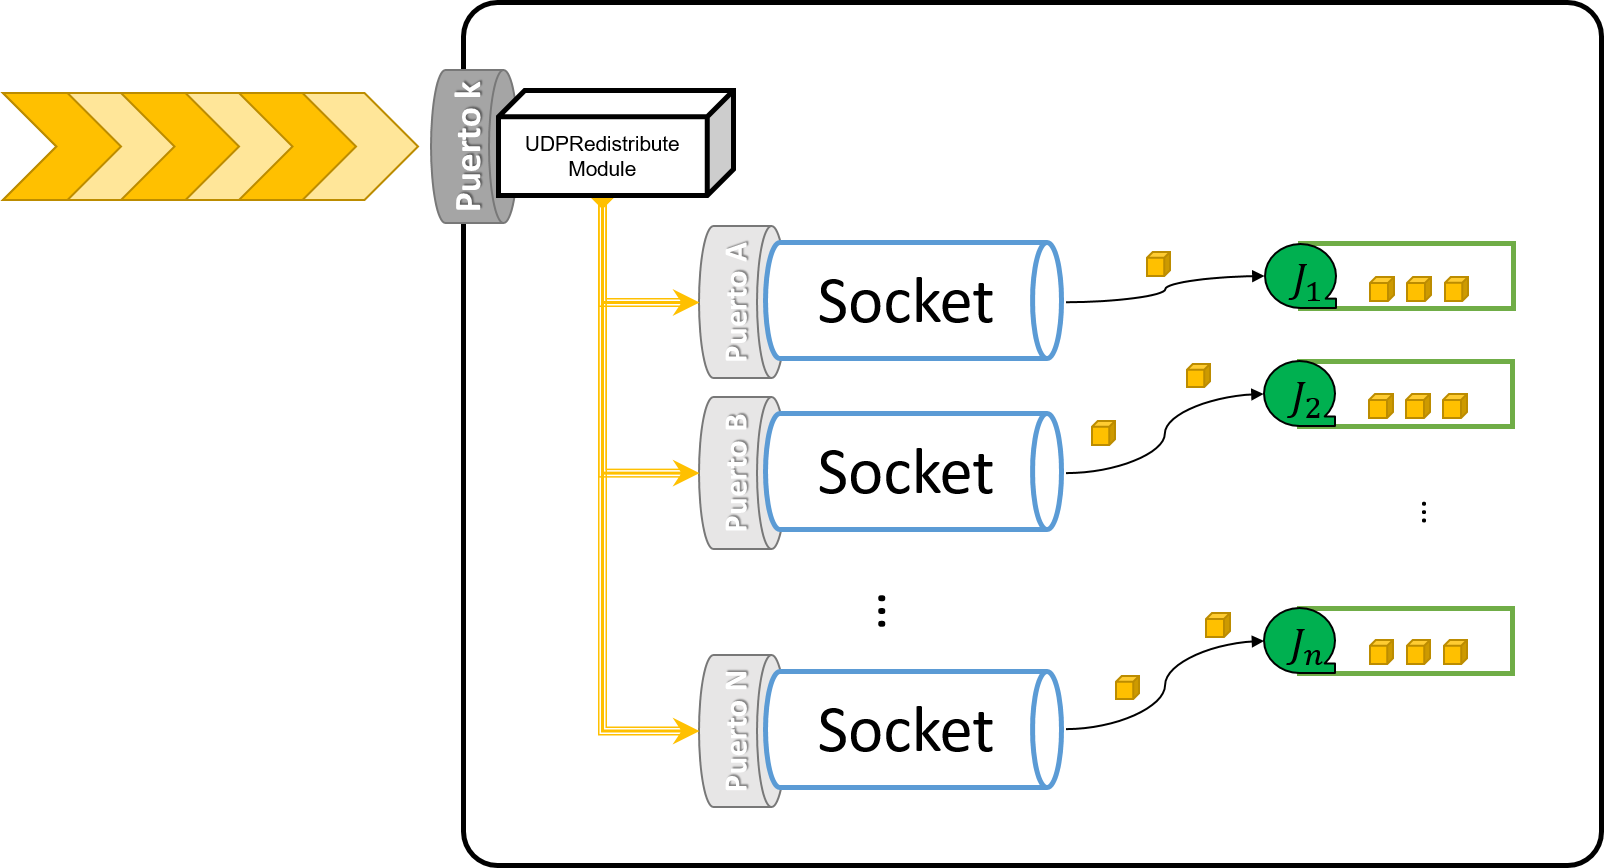
\includegraphics[scale=.5]{imagenes/adaptacioncasoestudio.png}
	\caption{Adaptación del esquema de la prueba UDP en un sistema con la solución desarrollada habilitada, correspondiente al nuevo caso de estudio.}
	\label{fig:casoPruebaModulo}
\end{figure}

\subsection{Resultados}
A continuación se presentan los resultados de los tiempos registrados en el experimento correspondiente al nuevo caso de estudio.

\begin{figure}[h!]
	\centering
	\hspace*{\fill}
	\subfigure[]{
		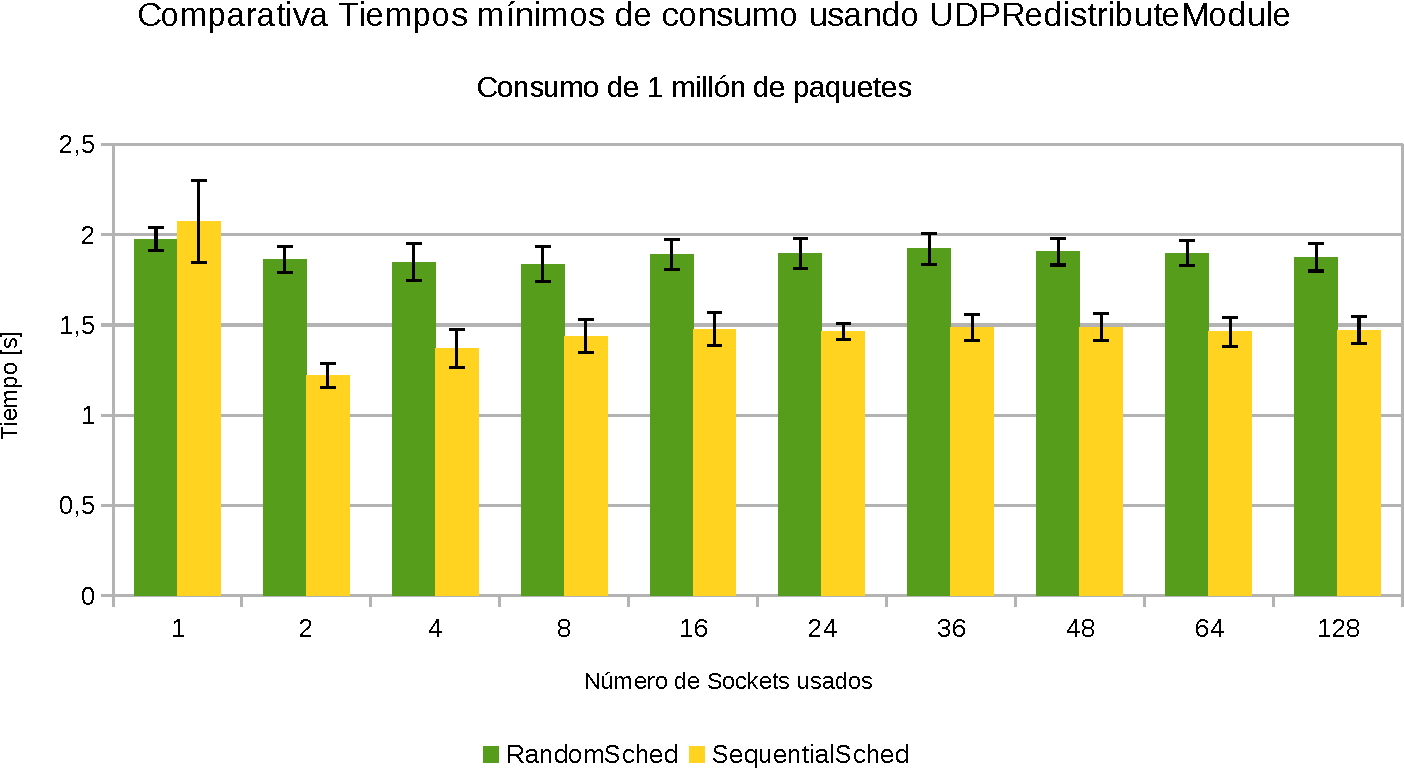
\includegraphics[width=.47\textwidth]{resultados/modulomin-crop.pdf}
		\label{fig:mimodulomin}
	}\hfill
	\subfigure[]{
		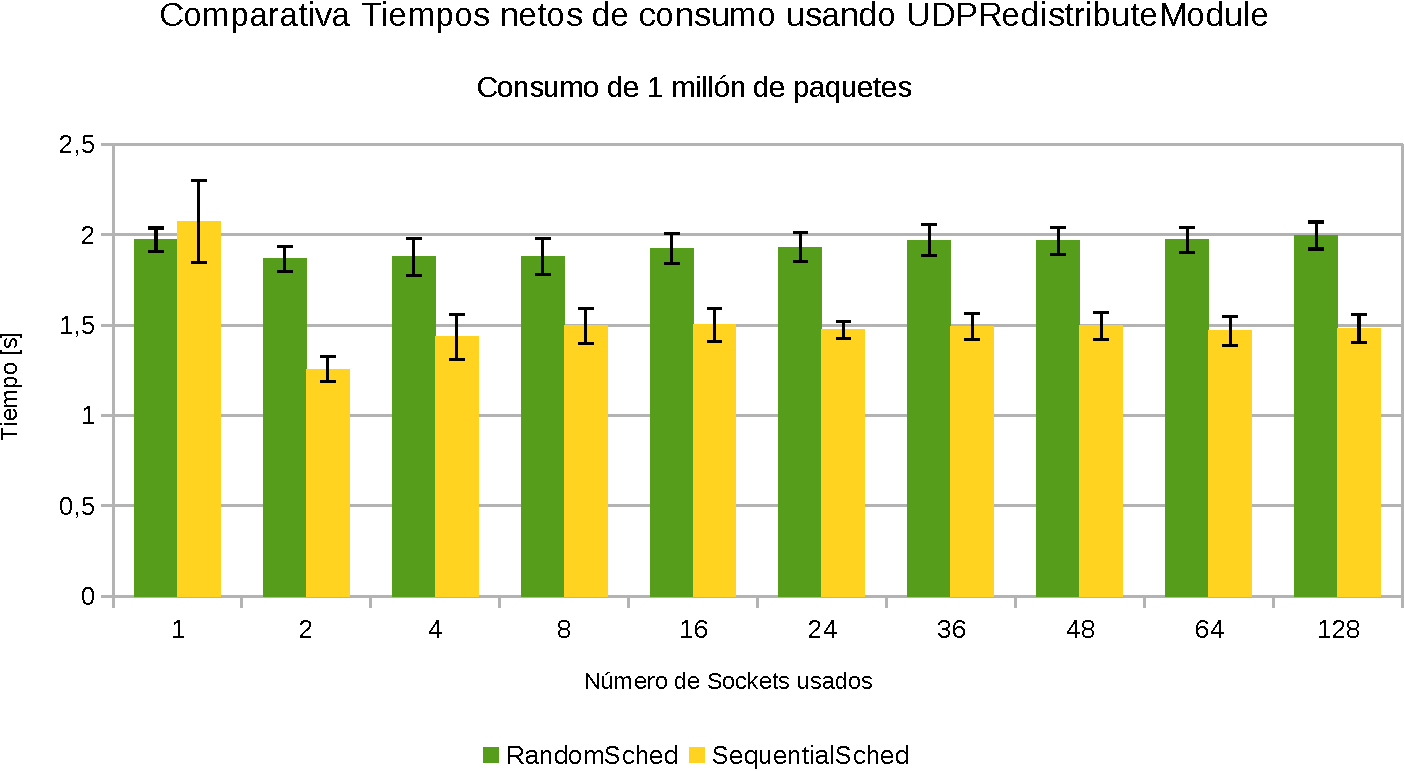
\includegraphics[width=.47\textwidth]{resultados/modulomax-crop.pdf}
		\label{fig:mimoduloneto}
	}
	\caption{Gráfico con tiempos de consumo del módulo solución \textbf{UDPRedistributeModule} para el nuevo caso de estudio.}
	\label{fig:resultadoMiModuloMinMax}
	\hspace*{\fill}
\end{figure}

En primera instancia, la solución consigue tanto en sus tiempos mínimos como netos una ganancia en el tiempo de la prueba usando múltiples sockets con respecto al caso de uso de un solo socket, algo nunca conseguido usando el enfoque de consumo concurrente sobre un socket usando múltiples hilos. Otro aspecto interesante es que el rendimiento de la solución usando el mecanismo de distribución \emph{SequentialSched} es más eficiente que el correspondiente con \emph{RandomSched}, situación comprensible entendiendo que por su naturaleza, el esquema secuencial satisface la cuota de los sockets alimentados sin desperdiciar ningún paquete, esto producto de tener una distribución totalmente justa entre sockets. Diferencia crucial con respecto al esquema de distribución aleatorio donde se puede dar el caso de que los sockets no reciban una cuota idéntica, pudiendo así cumplir algunos su cuota primero y causando la perdida paquetes al redirigidos a sockets satisfechos en la prueba.

Por otro lado, los tiempos netos de transferencia registran un decrecimiento constante a medida que se usan más sockets, similar a la tendencia obtenida con la opción \emph{Reuseport} lo cual sugiere un comportamiento posiblemente competitivo. Sin embargo, para evaluar el verdadero desempeño de la solución, es preciso comparar su rendimiento con otros escenarios y herramientas ya estudiadas.

\section{Comparación de Rendimiento}

avisar de los tiempos netos registrados en cada caso. destacar que, tal como reuseport, la solución implementada en cualquiera de sus dos esquemas de dsitribución brinda una ganancia efectiva con respecti al uso de threads y la postula como una alternativa a usar. más allá de que las variaciones entre los 3 ganadores existan, los 3 dan garantias de mejroes tiempos en el nuevo caso de estudio.

\begin{figure}[!h]
	\centering
	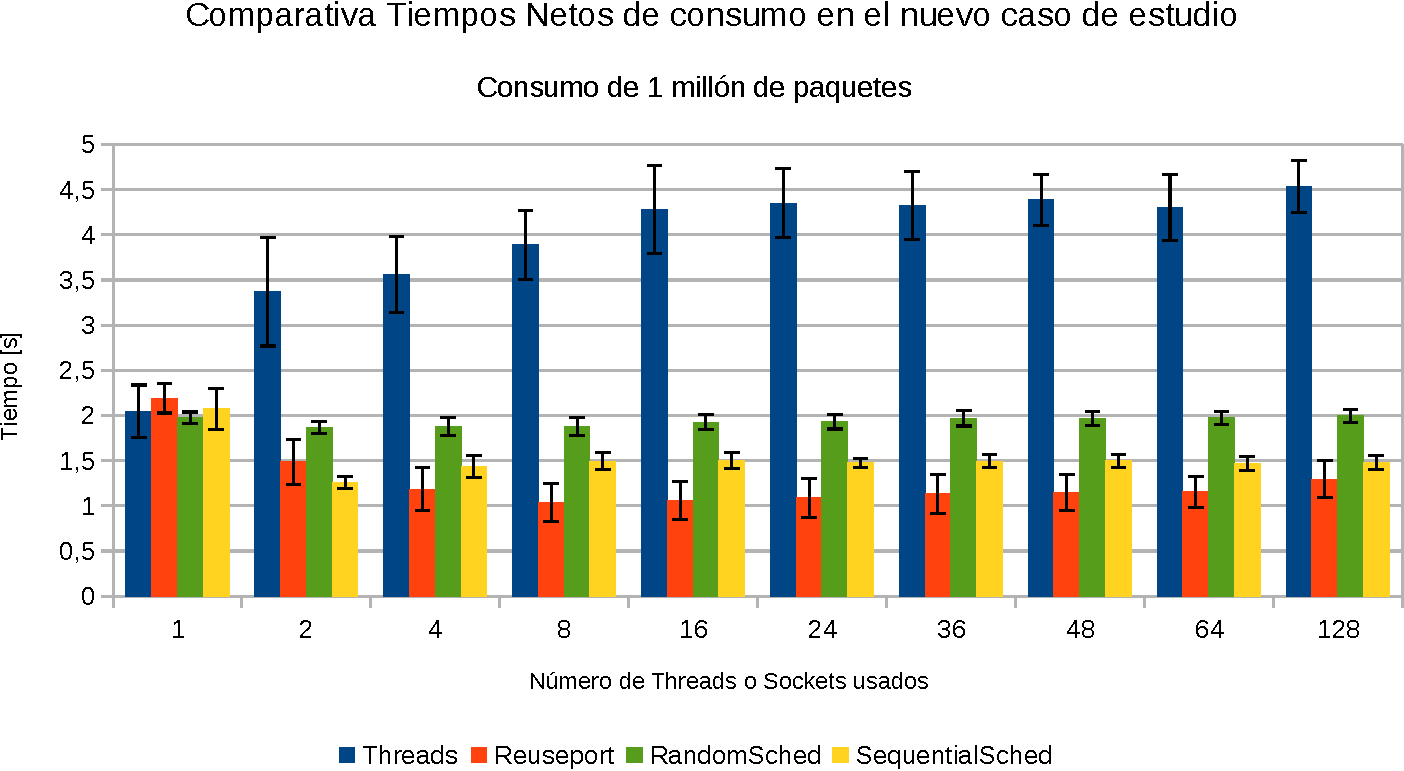
\includegraphics[scale=.6]{resultados/modulovstodos1-crop.pdf}
	\caption{Comparación de tiempos netos de consumo para el nuevo caso de estudio de todas las opciones de consumo estudiadas.}
	\label{fig:resultadoMiModulovsTodos}
\end{figure}

No obstante el resultado anterior, si rememoramos los resultados registrados por cada mecanísmo, notamos que existe un valor que diferencia notablemente a reuseport con respecto a nuestra solución (en cualquiera de sus dos sabores). Dicha diferencia viene dada por la variación que presenta cada mecanísmo entre los tiempos minimos y tiempos netos que registra. Para ilustrar mejor lo anterior, definimos el \textbf{tiempo de coordinación} como el tiempo transcurrido entre el tiempo neto y el tiempo mínimo registrado en la prueba. De la misma manera, definimos un proporcional porcentual del tiempo de coordinación con respecto al tiempo neto de la prueba como \textbf{indice de coordinación} con el simbolo $\eta$, de acuerdo a la siguiente ecuación:

\begin{equation}
\eta = \frac{\left(Tº Neto - Tº Mínimo\right)}{Tº Neto}
\end{equation}

De esta forma, el indice de coordinación ilustra la variación entre la finalización de trabajo de cada socket con respecto al tiempo total de la prueba misma. 

En la práctica, cuando $\eta\rightarrow 0$ indica que los tiempos de los distintos sockets trabajando son equitativos, y la prueba la completan todos de forma simultanea. Al contrario, cuando ocurre que $\eta \rightarrow 1$ indica que los distintos sockets terminan su trabajo en tiempos muy diferentes entre sí, más aún, indica que todo el tiempo neto de la prueba se está debiendo a la actividad del último socket en ternminar, habiendo finalizado los demás hace mucho.

A continuación se presentan los resultados del indice de coordinación para los distintos mecanísmos estudiados en ésta investigación.

\begin{figure}[!h]
	\centering
	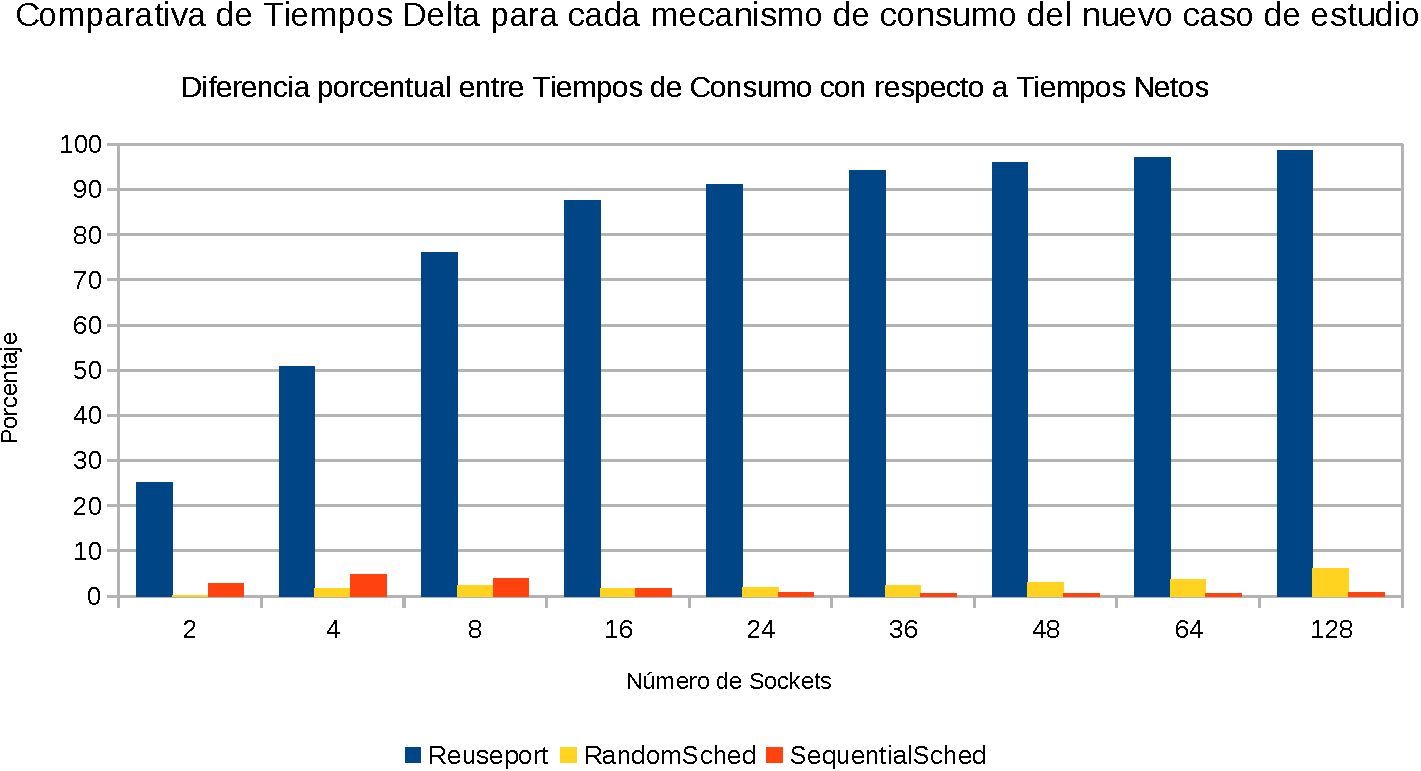
\includegraphics[scale=.6]{resultados/tiempodelta-crop.pdf}
	\caption{Comparativa de tiempos .}
	\label{fig:tiemposdelta}
\end{figure}


\section{Aciertos de la solución}

A raíz de los análisis anteriores, se desprenden varios aspectos rescatables de la solución implementada, obtenidos como consecuencia de satisfacer los requerimientos de operación planteados al comienzo del presente capítulo, y que diferencian neustra solución de las opciones disponibles.

Un primer elemento a destacar es el \textbf{rendimiento}. En las pruebas desarrolladas en secciones anteriores se corroboró la efectividad de la solución propuesta, comparándola con la mejor alternativa disponible: \emph{Reuseport}, de donde se concluyó que nuestra propuesta logra un comportamiento similar al de \emph{Reuseport} en terminos nominales, conservando un margen de diferencias que mantiene a \emph{Reuseport} como la opción más rápida, pero postulando nuestro desarrollo como competitivo en esa linea.

Un segundo punto a destacar de la solución es su \textbf{equitatividad de tiempos}, una característica que lo diferencia de \emph{Reuseport} pues, nuestro diseño provee un rendimiento más homogéneo entre múltiples procesos. Ésta característica es muy interesante de resaltar pues hay aplicaciones donde es necesario garantizar un escenario altamente \emph{Fairness} y experimentalmente nuestra solución luce prometedora en ese sentido.

Otro aspecto a destacar de nuestra solución es que logra buenos rendimientos preservando los \textbf{principios de diseño del modelo OSI}. Ésta característica era fundamental de proveer pues da garantías de facil adopción de la solución en entornos con aplicaciones ya operativas sin mayores modificaciones de los mismos.

El último y más importante acierto a reconocer de neustra solución consiste en su \textbf{configurabilidad} y \textbf{extensibilidad}. El primero pues, cómo se explicó en secciones anteriores, la solución admite distintos parámetros de configuración que permiten, sin cambios del código fuente, proveer distintos modos de funcionamiento según el requerimiento de consumo y distribución que se busque. El segundo dado por la implementación misma de la solución, ello pues al ser un módulo del kernel, es facilmente modificable para añadir nuevo código fuente que permita modificar los esquemas de distribución, etapas de interceptación de paquetes, funcionamiento del framework de \emph{Netfilters}, etc.

\section{Proyecciones}
La solución planteada en la presente investigación cumple correctamente para los fines con que se postuló originalmente, basada en su satisfacción de los requerimientos especificados en la seccion previa. Sin embargo, el mismo modelo de operación que se planteó en ésta solución puede ser aprovechado y extendido para ser usado en otros escenarios o contextos.

Un caso interesante consiste en extender la solución para funcionar con otros protocolos orientados a la conexión, como por ejemplo TCP. El gran problema de la solución desarrollada para con el caso de TCP es salvar correctamente la etapa de negociación inicial para establecer la conexión -El denominado \emph{Handshake} de TCP-. En este contexto, la solución desarrollada debe poder contemplar un mecanismo para poder hacer una correcta redistribución de paquetes para respetar la asignación apropiada entre los paquetes recibidos y las conexiones que se están llevando a cabo.

Gracias a su buen diseño, suplir el requerimiento anterior es sencillo con nuestra solución. Basta implementar un nuevo esquema de distribución que sea conciente de la distribución de paquetes para, usando las tuplas de datos de origen/destino de cada paquete, hacer una distribución correcta entre los sockets de redirección, para que las conexiones sean correctas. Para ello, una solución interesante es en lugar de aplicar un criterio aleatorio o secuencial de distribución como se usó en los esquemas provistos en éste trabajo, emplear una \emph{función de Hash} que use las tuplas de origen/destino de cada paquete y así, lleve un registro lógico correcto de las conexiones que están operativas sobre un mismo socket.

\begin{figure}[!h]
	\centering
	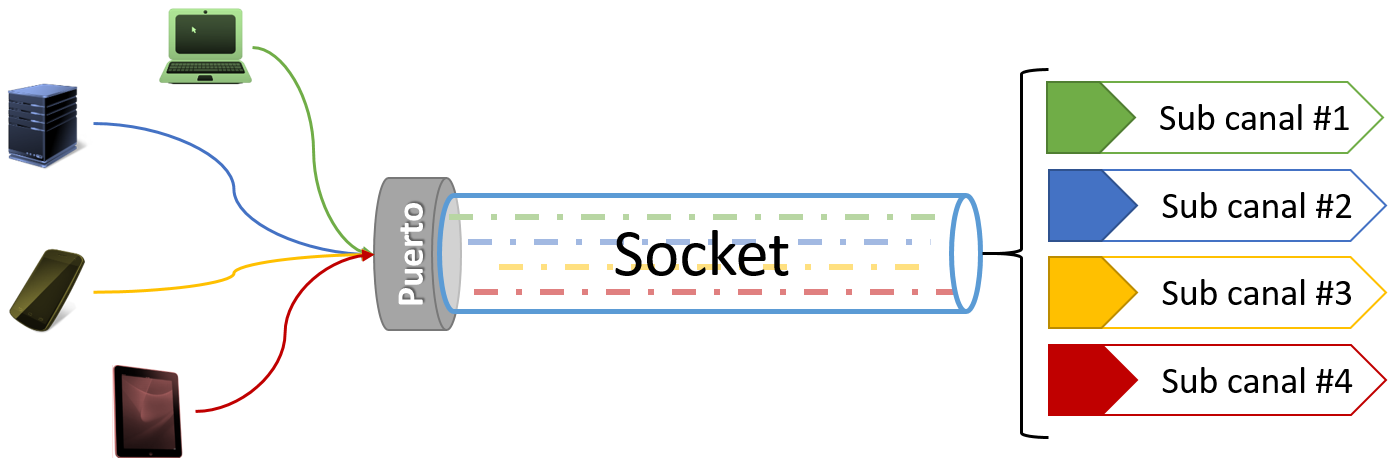
\includegraphics[scale=.5]{imagenes/socketMultiplexed.png}
	\caption{Capacidad de multiplexar un único puerto lógico del sistema, permitiendo comunicación diversa en una única interfaz de red.}
	\label{fig:multiplexarPuerto}
\end{figure}

El enfoque antes planteado es sumamente poderoso y brinda una interesante oportunidad puespostula la capacidad de \textbf{multiplexar} un único puerto del sistema, haciendo posible la recepción de paquetes genéricos en una misma interfaz y reasignar los mismos a un pool de otros sockets atendidos por aplicaciones independientes. En otras palabras, se podrían atender diversos requerimientos en una misma interfaz lógica del sistema asociada a un puerto para atender una variedad de servicios, rigiendo la distribución según las características mismas de un paquete (Ver imagen \ref{fig:multiplexarPuerto}).

Tan flexible es éste enfoque que permite soportar una diversidad de servicios (ya sean orientados a la conexión o a la mensajería) sobre una única interfaz lógica de conexión según las capas 3 y 4 del modelo OSI. Ésto en la práctica permite postular a mejoras en aspectos como seguridad, permitiendo que sólo los servicios reconocidos consiguen realizar conexiones correctas. Un ejemplo práctico de ello anterior se ilustra en la imagen \ref{fig:multiplexarPuertoEjemplo} donde se muestran distintas aplicaciones que operan trabajando con paquetes de diversa naturaleza (tanto por sus características, como por sus orígenes) pudiendo reasignar, clonar o simplemente descartar paquetes, según la naturaleza de las reglas definidas en el módulo.

\begin{figure}[!h]
	\centering
	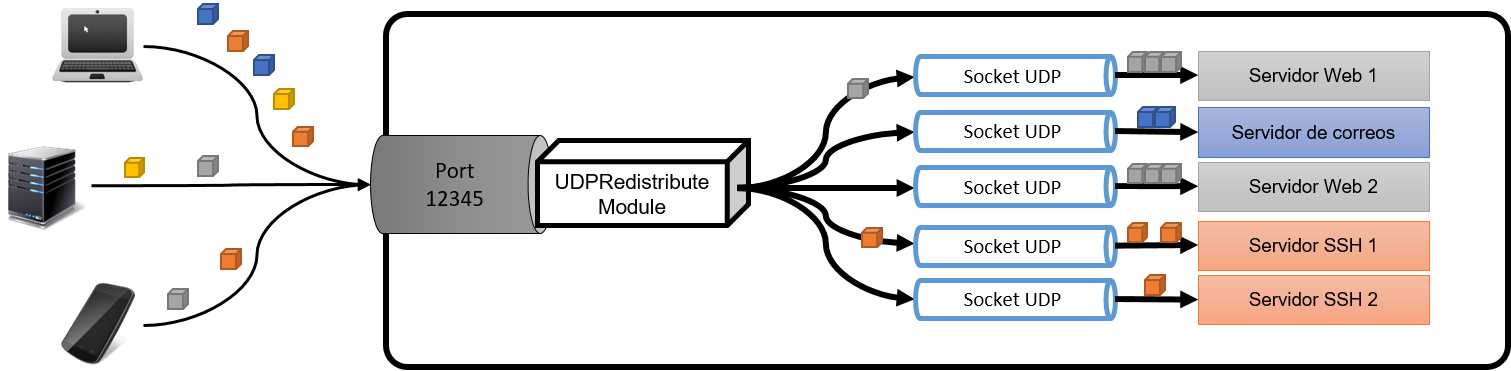
\includegraphics[scale=.6]{imagenes/udpredistributeapplications.png}
	\caption{Ejemplo de como multiplexar un puerto con varias aplicaciones diferentes. Es el módulo el encargado de la resolución de la entrega de paquetes según sus características internas.}
	\label{fig:multiplexarPuertoEjemplo}
\end{figure}
